% Options for packages loaded elsewhere
\PassOptionsToPackage{unicode}{hyperref}
\PassOptionsToPackage{hyphens}{url}
%
\documentclass[
]{article}
\usepackage{amsmath,amssymb}
\usepackage{lmodern}
\usepackage{iftex}
\ifPDFTeX
  \usepackage[T1]{fontenc}
  \usepackage[utf8]{inputenc}
  \usepackage{textcomp} % provide euro and other symbols
\else % if luatex or xetex
  \usepackage{unicode-math}
  \defaultfontfeatures{Scale=MatchLowercase}
  \defaultfontfeatures[\rmfamily]{Ligatures=TeX,Scale=1}
\fi
% Use upquote if available, for straight quotes in verbatim environments
\IfFileExists{upquote.sty}{\usepackage{upquote}}{}
\IfFileExists{microtype.sty}{% use microtype if available
  \usepackage[]{microtype}
  \UseMicrotypeSet[protrusion]{basicmath} % disable protrusion for tt fonts
}{}
\makeatletter
\@ifundefined{KOMAClassName}{% if non-KOMA class
  \IfFileExists{parskip.sty}{%
    \usepackage{parskip}
  }{% else
    \setlength{\parindent}{0pt}
    \setlength{\parskip}{6pt plus 2pt minus 1pt}}
}{% if KOMA class
  \KOMAoptions{parskip=half}}
\makeatother
\usepackage{xcolor}
\usepackage[margin=1in]{geometry}
\usepackage{color}
\usepackage{fancyvrb}
\newcommand{\VerbBar}{|}
\newcommand{\VERB}{\Verb[commandchars=\\\{\}]}
\DefineVerbatimEnvironment{Highlighting}{Verbatim}{commandchars=\\\{\}}
% Add ',fontsize=\small' for more characters per line
\usepackage{framed}
\definecolor{shadecolor}{RGB}{248,248,248}
\newenvironment{Shaded}{\begin{snugshade}}{\end{snugshade}}
\newcommand{\AlertTok}[1]{\textcolor[rgb]{0.94,0.16,0.16}{#1}}
\newcommand{\AnnotationTok}[1]{\textcolor[rgb]{0.56,0.35,0.01}{\textbf{\textit{#1}}}}
\newcommand{\AttributeTok}[1]{\textcolor[rgb]{0.77,0.63,0.00}{#1}}
\newcommand{\BaseNTok}[1]{\textcolor[rgb]{0.00,0.00,0.81}{#1}}
\newcommand{\BuiltInTok}[1]{#1}
\newcommand{\CharTok}[1]{\textcolor[rgb]{0.31,0.60,0.02}{#1}}
\newcommand{\CommentTok}[1]{\textcolor[rgb]{0.56,0.35,0.01}{\textit{#1}}}
\newcommand{\CommentVarTok}[1]{\textcolor[rgb]{0.56,0.35,0.01}{\textbf{\textit{#1}}}}
\newcommand{\ConstantTok}[1]{\textcolor[rgb]{0.00,0.00,0.00}{#1}}
\newcommand{\ControlFlowTok}[1]{\textcolor[rgb]{0.13,0.29,0.53}{\textbf{#1}}}
\newcommand{\DataTypeTok}[1]{\textcolor[rgb]{0.13,0.29,0.53}{#1}}
\newcommand{\DecValTok}[1]{\textcolor[rgb]{0.00,0.00,0.81}{#1}}
\newcommand{\DocumentationTok}[1]{\textcolor[rgb]{0.56,0.35,0.01}{\textbf{\textit{#1}}}}
\newcommand{\ErrorTok}[1]{\textcolor[rgb]{0.64,0.00,0.00}{\textbf{#1}}}
\newcommand{\ExtensionTok}[1]{#1}
\newcommand{\FloatTok}[1]{\textcolor[rgb]{0.00,0.00,0.81}{#1}}
\newcommand{\FunctionTok}[1]{\textcolor[rgb]{0.00,0.00,0.00}{#1}}
\newcommand{\ImportTok}[1]{#1}
\newcommand{\InformationTok}[1]{\textcolor[rgb]{0.56,0.35,0.01}{\textbf{\textit{#1}}}}
\newcommand{\KeywordTok}[1]{\textcolor[rgb]{0.13,0.29,0.53}{\textbf{#1}}}
\newcommand{\NormalTok}[1]{#1}
\newcommand{\OperatorTok}[1]{\textcolor[rgb]{0.81,0.36,0.00}{\textbf{#1}}}
\newcommand{\OtherTok}[1]{\textcolor[rgb]{0.56,0.35,0.01}{#1}}
\newcommand{\PreprocessorTok}[1]{\textcolor[rgb]{0.56,0.35,0.01}{\textit{#1}}}
\newcommand{\RegionMarkerTok}[1]{#1}
\newcommand{\SpecialCharTok}[1]{\textcolor[rgb]{0.00,0.00,0.00}{#1}}
\newcommand{\SpecialStringTok}[1]{\textcolor[rgb]{0.31,0.60,0.02}{#1}}
\newcommand{\StringTok}[1]{\textcolor[rgb]{0.31,0.60,0.02}{#1}}
\newcommand{\VariableTok}[1]{\textcolor[rgb]{0.00,0.00,0.00}{#1}}
\newcommand{\VerbatimStringTok}[1]{\textcolor[rgb]{0.31,0.60,0.02}{#1}}
\newcommand{\WarningTok}[1]{\textcolor[rgb]{0.56,0.35,0.01}{\textbf{\textit{#1}}}}
\usepackage{graphicx}
\makeatletter
\def\maxwidth{\ifdim\Gin@nat@width>\linewidth\linewidth\else\Gin@nat@width\fi}
\def\maxheight{\ifdim\Gin@nat@height>\textheight\textheight\else\Gin@nat@height\fi}
\makeatother
% Scale images if necessary, so that they will not overflow the page
% margins by default, and it is still possible to overwrite the defaults
% using explicit options in \includegraphics[width, height, ...]{}
\setkeys{Gin}{width=\maxwidth,height=\maxheight,keepaspectratio}
% Set default figure placement to htbp
\makeatletter
\def\fps@figure{htbp}
\makeatother
\setlength{\emergencystretch}{3em} % prevent overfull lines
\providecommand{\tightlist}{%
  \setlength{\itemsep}{0pt}\setlength{\parskip}{0pt}}
\setcounter{secnumdepth}{-\maxdimen} % remove section numbering
\usepackage{booktabs}
\usepackage{longtable}
\usepackage{array}
\usepackage{multirow}
\usepackage{wrapfig}
\usepackage{float}
\usepackage{colortbl}
\usepackage{pdflscape}
\usepackage{tabu}
\usepackage{threeparttable}
\usepackage{threeparttablex}
\usepackage[normalem]{ulem}
\usepackage{makecell}
\usepackage{xcolor}
\ifLuaTeX
  \usepackage{selnolig}  % disable illegal ligatures
\fi
\IfFileExists{bookmark.sty}{\usepackage{bookmark}}{\usepackage{hyperref}}
\IfFileExists{xurl.sty}{\usepackage{xurl}}{} % add URL line breaks if available
\urlstyle{same} % disable monospaced font for URLs
\hypersetup{
  pdftitle={41903 Pset 3},
  pdfauthor={Andrew McKinley, Lauren Mostrom, Pietro Ramella, Francisco Ruela, and Bohan Yang},
  hidelinks,
  pdfcreator={LaTeX via pandoc}}

\title{41903 Pset 3}
\author{Andrew McKinley, Lauren Mostrom, Pietro Ramella, Francisco
Ruela, and Bohan Yang}
\date{May 12, 2022}

\begin{document}
\maketitle

\hypertarget{question-1}{%
\subsection{Question 1}\label{question-1}}

\hypertarget{a}{%
\subsubsection{(a)}\label{a}}

Adding aggregate time effects captures macro trends that affects all
countries in certain periods, for example a recession that interests all
countries in a given year.

\hypertarget{b}{%
\subsubsection{(b)}\label{b}}

The country fixed effects \(\alpha_i\) capture unobserved heterogeneity
that is constant within country over the examined period, for example
levels of natural resources, or institutional factors.

\hypertarget{c}{%
\subsubsection{(c)}\label{c}}

Economic reasoning suggests a negative \(\delta_1\): because higher tax
rates makes investment less profitable, we would expect that a decrease
in investment would follow higher marginal tax rates.

\hypertarget{d}{%
\subsubsection{(d)}\label{d}}

Rewrite the model in matrix form:
\[Y = \theta R + \alpha D + \gamma Z + \delta_1 tax + \delta_2 disaster + u = \alpha D + \beta X + u\]
where
\(Y_{it} = log(investment_{it}),\ \beta = [\delta_1, \delta_2, \gamma', \theta'],\ X = [tax',disaster',Z',R']'\).\textbackslash{}
Because fixed effects, \(\delta = [\delta_1,\delta_2]\), and an
intercept cannot be jointly identified, I need to choose a
normalization: set to zero the intercept and the first time fixed
effect. If we are willing to assume strict exogeneity, that is \(tax\)
and \(disaster\) are uncorrelated with \(\epsilon\) at every time
period, we can then estimate using OLS the coefficients
\[(\hat{\beta}_{FE},\hat{\alpha})=(W'W )^{-1}(W'Y)\] where
\(W=[X\ D]\).\textbackslash{} To compute the standard errors, assuming
observations are independent across countries,
\(\hat{V} = \hat{\sigma}^2\hat{Q}^{-1}\), where
\[\hat{\sigma}^2=\frac{1}{NT}\sum_{i,t}e_{it}^2, \quad e_{it} = y_{it} - \Bar{y}_i - (x_{it} - \Bar{x}_i)'\hat{\beta}_{FE},\ k=dim(x_{it})\]
\[\hat{Q} = \frac{1}{NT}\sum_{i,t} (x_{it} - \Bar{x}_i)(x_{it} - \Bar{x}_i)'\].

\hypertarget{e}{%
\subsubsection{(e)}\label{e}}

It seems unlikely that we can rule out dynamics between new capital
investments and changes in marginal taxes or natural disasters, yet,
\(tax_{it}\) may still violate strict exogeneity because the taxing
authority may choose \(tax_{it}\) in response of low/excessive levels of
observed investment, therefore \(E[x_{it},u{it-j}]\ne0\) for some
\(j=1,..\). There are not real issues with natural disasters if we rule
out persistent effects, and therefore dynamics.

\newpage

\hypertarget{question-2}{%
\subsection{Question 2}\label{question-2}}

\hypertarget{a-1}{%
\subsubsection{(a)}\label{a-1}}

\begin{Shaded}
\begin{Highlighting}[]
\CommentTok{\#setwd("C:/Users/17036/OneDrive/Documents/GitHub/metrics3{-}zombie{-}boards/Psets/3")}
\NormalTok{murder }\OtherTok{\textless{}{-}} \FunctionTok{read.delim}\NormalTok{(}\StringTok{"PS3Data/MURDER\_RAW.txt"}\NormalTok{, }\AttributeTok{header=}\ConstantTok{FALSE}\NormalTok{)}

\FunctionTok{colnames}\NormalTok{(murder) }\OtherTok{\textless{}{-}} \FunctionTok{c}\NormalTok{(}\StringTok{\textquotesingle{}id\textquotesingle{}}\NormalTok{,}\StringTok{\textquotesingle{}state\textquotesingle{}}\NormalTok{,}\StringTok{\textquotesingle{}year\textquotesingle{}}\NormalTok{,}\StringTok{\textquotesingle{}mrdrte\textquotesingle{}}\NormalTok{,}\StringTok{\textquotesingle{}exec\textquotesingle{}}\NormalTok{,}\StringTok{\textquotesingle{}unem\textquotesingle{}}\NormalTok{,}\StringTok{\textquotesingle{}d90\textquotesingle{}}\NormalTok{,}\StringTok{\textquotesingle{}d93\textquotesingle{}}\NormalTok{,      }
                      \StringTok{\textquotesingle{}cmrdrte\textquotesingle{}}\NormalTok{,}\StringTok{\textquotesingle{}cexec\textquotesingle{}}\NormalTok{,}\StringTok{\textquotesingle{}cunem\textquotesingle{}}\NormalTok{,}\StringTok{\textquotesingle{}cexec1\textquotesingle{}}\NormalTok{,}\StringTok{\textquotesingle{}cunem1\textquotesingle{}}\NormalTok{)}

\CommentTok{\# Use only data for 1990 and 1993}
\NormalTok{data }\OtherTok{\textless{}{-}}\NormalTok{ murder }\SpecialCharTok{\%\textgreater{}\%}
  \FunctionTok{filter}\NormalTok{(year}\SpecialCharTok{==}\DecValTok{90} \SpecialCharTok{|}\NormalTok{ year}\SpecialCharTok{==}\DecValTok{93}\NormalTok{)}

\NormalTok{reg\_pooled }\OtherTok{\textless{}{-}} \FunctionTok{lm}\NormalTok{(mrdrte}\SpecialCharTok{\textasciitilde{}}\NormalTok{d93}\SpecialCharTok{+}\NormalTok{exec}\SpecialCharTok{+}\NormalTok{unem, }\AttributeTok{data=}\NormalTok{data)}
\DocumentationTok{\#\#\# calculate standard errors }
\CommentTok{\# standard homoskedastic standard errors}
\NormalTok{se.homo\_pooled }\OtherTok{\textless{}{-}} \FunctionTok{sqrt}\NormalTok{(}\FunctionTok{diag}\NormalTok{(}\FunctionTok{vcov}\NormalTok{(reg\_pooled))) }
\CommentTok{\# robust standard errors}
\NormalTok{HCV.coef\_pooled }\OtherTok{\textless{}{-}} \FunctionTok{vcovHC}\NormalTok{(reg\_pooled, }\AttributeTok{type =} \StringTok{\textquotesingle{}HC1\textquotesingle{}}\NormalTok{)}
\NormalTok{se.robust\_pooled }\OtherTok{\textless{}{-}} \FunctionTok{sqrt}\NormalTok{(}\FunctionTok{diag}\NormalTok{(HCV.coef\_pooled)) }
\CommentTok{\# clustered standard errors}
\NormalTok{CLCV.coef\_pooled }\OtherTok{\textless{}{-}} \FunctionTok{cluster.vcov}\NormalTok{(reg\_pooled,data}\SpecialCharTok{$}\NormalTok{state)}
\NormalTok{se.cluster\_pooled }\OtherTok{\textless{}{-}} \FunctionTok{sqrt}\NormalTok{(}\FunctionTok{diag}\NormalTok{(CLCV.coef\_pooled))}
\end{Highlighting}
\end{Shaded}

In the table below we report the IID standard errors,
heteroskedasticity-robust standard errors, and clustered standard
errors. Robust SEs were calculated as follows:

\[
\hat{\Omega} = \left( \frac{1}{NT} \sum_{i,t} x_{it} x_{it}'\right)^{-1} \left( \frac{1}{NT} \sum_{i,t} x_{it} x_{it}' \hat{\epsilon}_{it}^2 \right) \left( \frac{1}{NT} \sum_{i,t} x_{it} x_{it}'\right)^{-1}
\]

Where \(\hat{\epsilon}\) is the POLS residual. We also include clustered
standard errors; however, if we suspect the observations are serially
correlated (as would be implied by the use of clustered SEs) we should
not be using POLS anyway. Nevertheless, clustered SEs were calculated as
follows:

\[
\hat{\Omega} = \left( \frac{1}{NT} \sum_{i,t} x_{it} x_{it}'\right)^{-1} \left( \frac{1}{NT} \sum_{i,t}  x_{it} x_{i,90}' \hat{\epsilon}_{it} \hat{\epsilon}_{i,90} + x_{it} x_{i,93}' \hat{\epsilon}_{it} \hat{\epsilon}_{i,93} \right) \left( \frac{1}{NT} \sum_{i,t} x_{it} x_{it}'\right)^{-1}
\]

\newpage

\begin{Shaded}
\begin{Highlighting}[]
\FunctionTok{texreg}\NormalTok{(}\FunctionTok{list}\NormalTok{(reg\_pooled, reg\_pooled, reg\_pooled), }\AttributeTok{digits=}\DecValTok{4}\NormalTok{, }\AttributeTok{caption.above=}\ConstantTok{TRUE}\NormalTok{,}
       \AttributeTok{override.se =} \FunctionTok{list}\NormalTok{(se.homo\_pooled, se.robust\_pooled, se.cluster\_pooled),}
       \AttributeTok{custom.model.names=}\FunctionTok{c}\NormalTok{(}\StringTok{"IID"}\NormalTok{, }\StringTok{"Robust"}\NormalTok{, }\StringTok{"Clustered"}\NormalTok{),}
       \AttributeTok{caption =} \StringTok{"Pooled OLS"}\NormalTok{)}
\end{Highlighting}
\end{Shaded}

\begin{table}
\caption{Pooled OLS}
\begin{center}
\begin{tabular}{l c c c}
\hline
 & IID & Robust & Clustered \\
\hline
(Intercept) & $-5.2780$     & $-5.2780$     & $-5.2780$     \\
            & $(4.4278)$    & $(5.3868)$    & $(6.6760)$    \\
d93         & $-2.0674$     & $-2.0674$     & $-2.0674$     \\
            & $(2.1446)$    & $(1.9981)$    & $(1.3066)$    \\
exec        & $0.1277$      & $0.1277$      & $0.1277$      \\
            & $(0.2632)$    & $(0.1342)$    & $(0.1678)$    \\
unem        & $2.5289^{**}$ & $2.5289^{**}$ & $2.5289^{**}$ \\
            & $(0.7817)$    & $(1.1076)$    & $(1.5047)$    \\
\hline
R$^2$       & $0.1016$      & $0.1016$      & $0.1016$      \\
Adj. R$^2$  & $0.0741$      & $0.0741$      & $0.0741$      \\
Num. obs.   & $102$         & $102$         & $102$         \\
\hline
\multicolumn{4}{l}{\scriptsize{$^{***}p<0.001$; $^{**}p<0.01$; $^{*}p<0.05$}}
\end{tabular}
\label{table:coefficients}
\end{center}
\end{table}

\hypertarget{b-1}{%
\subsubsection{(b)}\label{b-1}}

In this setting FE and FD are numerically identical because there are
only two time periods, 1990 and 1993. To see this, recall the fixed
effect model:

\begin{align*}
  y_{i1} - \bar{y}_i &= (x_{i1} - \bar{x}_i)' \beta + \epsilon_{i1} - \bar{\epsilon}_i \\
  y_{i1} - \left( \frac{y_{i1}+y_{i0}}{2} \right) &= \left( x_{i1} - \frac{x_{i1}+x_{i0}}{2} \right)' \beta + \epsilon_{i1} - \left( \frac{\epsilon_{i1}+\epsilon_{i0}}{2} \right) \\
  \frac{y_{i1} - y_{i0}}{2} &= \left( \frac{x_{i1} - x_{i0}}{2} \right)' \beta + \frac{\epsilon_{i1} - \epsilon_{i0}}{2} \\
  y_{i1} - y_{i0} &= (x_{i1} - x_{i0})' \beta + \epsilon_{i1} - \epsilon_{i0}
\end{align*}

Which is exactly the first differences model.

In the table below we report only the results for FD. We chose FD
because it reduces the procedure down to a cross-sectional dataset and
only requires heterskedasticity-robust standard errors, rather than
maintaining the panel data structure and requiring clustered standard
errors. Clustered standard errors are reported in the table below, but
only to illustrate that they are identical to robust in the first
differences method when we only have two periods.

There does not appear to be any deterrant effect of capital punishment;
based on these results we fail to reject the null hypothesis that the
coefficient on \(exec\) is equal to zero.

\hypertarget{c-1}{%
\subsubsection{(c)}\label{c-1}}

\emph{First Differences}

\begin{Shaded}
\begin{Highlighting}[]
\NormalTok{data\_90 }\OtherTok{\textless{}{-}}\NormalTok{ data }\SpecialCharTok{\%\textgreater{}\%}
  \FunctionTok{filter}\NormalTok{(year}\SpecialCharTok{==}\DecValTok{90}\NormalTok{)}
\NormalTok{data\_93 }\OtherTok{\textless{}{-}}\NormalTok{ data }\SpecialCharTok{\%\textgreater{}\%}
  \FunctionTok{filter}\NormalTok{(year}\SpecialCharTok{==}\DecValTok{93}\NormalTok{)}
\NormalTok{data\_fd }\OtherTok{\textless{}{-}} \FunctionTok{left\_join}\NormalTok{(data\_90,data\_93,}\AttributeTok{by=}\FunctionTok{c}\NormalTok{(}\StringTok{"id"}\NormalTok{))}
\NormalTok{data\_fd}\SpecialCharTok{$}\NormalTok{delta\_mrdrte }\OtherTok{\textless{}{-}}\NormalTok{ data\_fd}\SpecialCharTok{$}\NormalTok{mrdrte.y}\SpecialCharTok{{-}}\NormalTok{data\_fd}\SpecialCharTok{$}\NormalTok{mrdrte.x}
\NormalTok{data\_fd}\SpecialCharTok{$}\NormalTok{delta\_exec }\OtherTok{\textless{}{-}}\NormalTok{ data\_fd}\SpecialCharTok{$}\NormalTok{exec.y}\SpecialCharTok{{-}}\NormalTok{data\_fd}\SpecialCharTok{$}\NormalTok{exec.x}
\NormalTok{data\_fd}\SpecialCharTok{$}\NormalTok{delta\_unem }\OtherTok{\textless{}{-}}\NormalTok{ data\_fd}\SpecialCharTok{$}\NormalTok{unem.y}\SpecialCharTok{{-}}\NormalTok{data\_fd}\SpecialCharTok{$}\NormalTok{unem.x}
\NormalTok{reg\_fd }\OtherTok{\textless{}{-}} \FunctionTok{lm}\NormalTok{(delta\_mrdrte}\SpecialCharTok{\textasciitilde{}}\NormalTok{delta\_exec}\SpecialCharTok{+}\NormalTok{delta\_unem, }\AttributeTok{data=}\NormalTok{data\_fd)}
\DocumentationTok{\#\#\# calculate standard errors }
\CommentTok{\# standard homoskedastic standard errors}
\NormalTok{se.homo\_fd }\OtherTok{\textless{}{-}} \FunctionTok{sqrt}\NormalTok{(}\FunctionTok{diag}\NormalTok{(}\FunctionTok{vcov}\NormalTok{(reg\_fd))) }
\CommentTok{\# robust standard errors}
\NormalTok{HCV.coef\_fd }\OtherTok{\textless{}{-}} \FunctionTok{vcovHC}\NormalTok{(reg\_fd, }\AttributeTok{type =} \StringTok{\textquotesingle{}HC1\textquotesingle{}}\NormalTok{)}
\NormalTok{se.robust\_fd }\OtherTok{\textless{}{-}} \FunctionTok{sqrt}\NormalTok{(}\FunctionTok{diag}\NormalTok{(HCV.coef\_fd)) }
\CommentTok{\# clustered standard errors}
\NormalTok{CLCV.coef\_fd }\OtherTok{\textless{}{-}} \FunctionTok{cluster.vcov}\NormalTok{(reg\_fd,data\_fd}\SpecialCharTok{$}\NormalTok{state.x)}
\NormalTok{se.cluster\_fd }\OtherTok{\textless{}{-}} \FunctionTok{sqrt}\NormalTok{(}\FunctionTok{diag}\NormalTok{(CLCV.coef\_fd))}
\end{Highlighting}
\end{Shaded}

\newpage

\begin{Shaded}
\begin{Highlighting}[]
\FunctionTok{texreg}\NormalTok{(}\FunctionTok{list}\NormalTok{(reg\_fd, reg\_fd, reg\_fd), }\AttributeTok{digits=}\DecValTok{4}\NormalTok{, }\AttributeTok{caption.above=}\ConstantTok{TRUE}\NormalTok{,}
       \AttributeTok{override.se =} \FunctionTok{list}\NormalTok{(se.homo\_fd,se.robust\_fd,se.cluster\_fd),}
       \AttributeTok{custom.model.names=}\FunctionTok{c}\NormalTok{(}\StringTok{"IID"}\NormalTok{, }\StringTok{"Robust"}\NormalTok{, }\StringTok{"Clustered"}\NormalTok{),}
       \AttributeTok{caption =} \StringTok{"First Differences"}\NormalTok{)}
\end{Highlighting}
\end{Shaded}

\begin{table}
\caption{First Differences}
\begin{center}
\begin{tabular}{l c c c}
\hline
 & IID & Robust & Clustered \\
\hline
(Intercept) & $0.4133$      & $0.4133$      & $0.4133$      \\
            & $(0.2094)$    & $(0.2000)$    & $(0.2000)$    \\
delta\_exec & $-0.1038^{*}$ & $-0.1038^{*}$ & $-0.1038^{*}$ \\
            & $(0.0434)$    & $(0.0170)$    & $(0.0170)$    \\
delta\_unem & $-0.0666$     & $-0.0666$     & $-0.0666$     \\
            & $(0.1587)$    & $(0.1469)$    & $(0.1469)$    \\
\hline
R$^2$       & $0.1097$      & $0.1097$      & $0.1097$      \\
Adj. R$^2$  & $0.0727$      & $0.0727$      & $0.0727$      \\
Num. obs.   & $51$          & $51$          & $51$          \\
\hline
\multicolumn{4}{l}{\scriptsize{$^{***}p<0.001$; $^{**}p<0.01$; $^{*}p<0.05$}}
\end{tabular}
\label{table:coefficients}
\end{center}
\end{table}

As explained above, we used heteroskedasticity-robust SEs because the
assumptions required for IID standard errors are too strong, and in a
first differences model with only two periods, clustered and robust SEs
are identical (as demonstrated in the table above).

From these results the coefficient on \(exec\) is negative and
statistically significant, so it does appear that there is a deterrant
effect of capital punishment.

\hypertarget{d-1}{%
\subsubsection{(d)}\label{d-1}}

FD is preferred in this context because POLS requires the assumption
that there is no serial correlation between observations. This is an
unrealistic assumption in this setting because there could be many
persistent features of states that are correlated both with executions
and with the murder rate.

\newpage

\hypertarget{question-3}{%
\subsection{Question 3}\label{question-3}}

\textit{Compute the bias and root-mean-squared-error of each estimator. Form a histogram for each estimator. Do the histograms appear to be approximately normal centered over the true parameter value? Comment on what you think you learn that is generalizable from
this exercise.}

First, we include the tables of the bias and RMSE for the instance where
T = 6.

\begin{table}[!htbp] \centering 
  \caption{T=6} 
  \label{} 
\begin{tabular}{@{\extracolsep{5pt}} D{.}{.}{-3} D{.}{.}{-3} D{.}{.}{-3} D{.}{.}{-3} D{.}{.}{-3} } 
\\[-1.8ex]\hline 
\hline \\[-1.8ex] 
\multicolumn{1}{c}{} & \multicolumn{1}{c}{Fixed-Effects} & \multicolumn{1}{c}{First-Difference} & \multicolumn{1}{c}{Hahn-Kuersteiner} & \multicolumn{1}{c}{Jackknife} \\ 
\hline \\[-1.8ex] 
\multicolumn{1}{c}{Bias\_rho=  0} & -0.164 & 0.006 & -0.025 & 0.006 \\ 
\multicolumn{1}{c}{Bias\_rho = 0.5} & -0.260 & 0.007 & -0.054 & 0.148 \\ 
\multicolumn{1}{c}{Bias\_rho = 0.95} & -0.262 & 0.023 & 0.020 & 0.026 \\ 
\multicolumn{1}{c}{RMSE\_rho = 0} & 0.168 & 0.078 & 0.051 & 0.089 \\ 
\multicolumn{1}{c}{RMSE\_rho = 0.5} & 0.264 & 0.132 & 0.073 & 0.162 \\ 
\multicolumn{1}{c}{RMSE\_rho = 0.95} & 0.264 & 0.239 & 0.049 & 0.043 \\ 
\hline \\[-1.8ex] 
\end{tabular} 
\end{table}

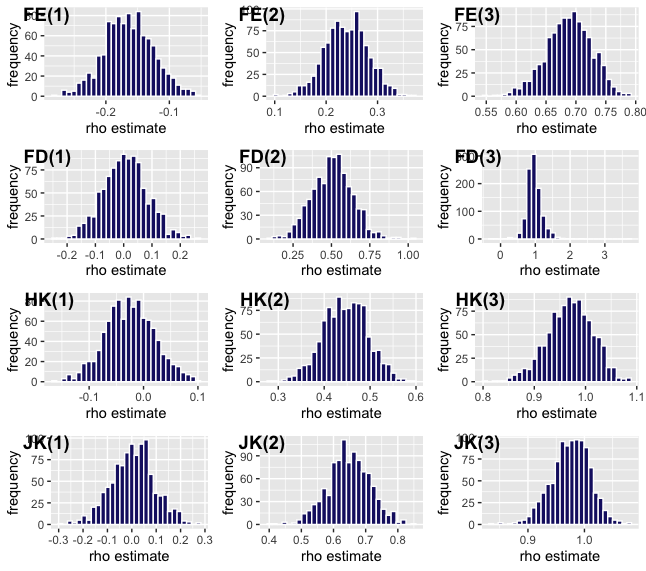
\includegraphics[scale=0.75]{PS3-Q3/T6 Plots.png}

Next, we include the same for the case where T = 25.

\begin{table}[!htbp] \centering 
  \caption{T=25} 
  \label{} 
\begin{tabular}{@{\extracolsep{5pt}} D{.}{.}{-3} D{.}{.}{-3} D{.}{.}{-3} D{.}{.}{-3} D{.}{.}{-3} } 
\\[-1.8ex]\hline 
\hline \\[-1.8ex] 
\multicolumn{1}{c}{} & \multicolumn{1}{c}{Fixed-Effects} & \multicolumn{1}{c}{First-Difference} & \multicolumn{1}{c}{Hahn-Kuersteiner} & \multicolumn{1}{c}{Jackknife} \\ 
\hline \\[-1.8ex] 
\multicolumn{1}{c}{Bias\_rho = 0} & -0.040 & -0.0001 & -0.002 & -0.0004 \\ 
\multicolumn{1}{c}{Bias\_rho = 0.5} & -0.062 & 0.003 & -0.004 & 0.230 \\ 
\multicolumn{1}{c}{Bias\_rho = 0.95} & -0.045 & 0.003 & 0.031 & 0.049 \\ 
\multicolumn{1}{c}{RMSE\_rho = 0} & 0.045 & 0.031 & 0.021 & 0.046 \\ 
\multicolumn{1}{c}{RMSE\_rho = 0.5} & 0.064 & 0.040 & 0.020 & 0.231 \\ 
\multicolumn{1}{c}{RMSE\_rho = 0.95} & 0.046 & 0.068 & 0.032 & 0.049 \\ 
\hline \\[-1.8ex] 
\end{tabular} 
\end{table}

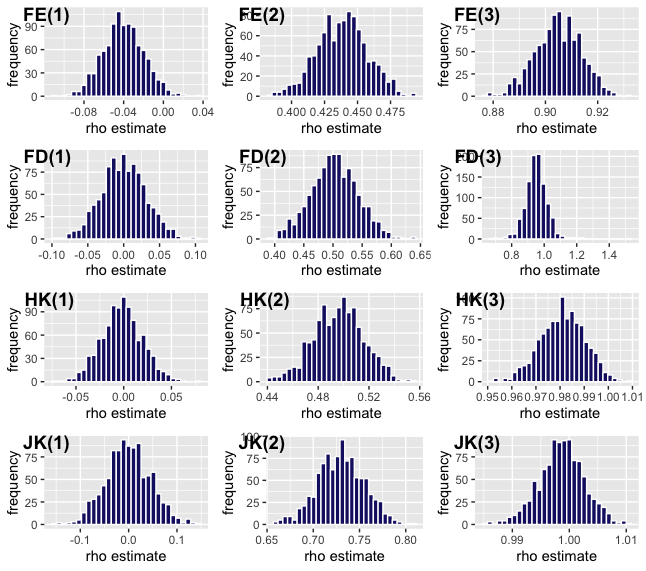
\includegraphics[scale=0.75]{PS3-Q3/T25.png}

We note that the distributions do appear to be approximately centered
over the true value in a few cases, notably those that are not the fixed
effects estimator which appears to have a wider spread and weaker
identification. However, some are still a bit off to either direction.
We can also see, as we learned in class, that as \(\frac{N}{T}\) gets
smaller that our inferences are better. In this case when T = 25.

It also appears that the First Difference IV estimator works better for
lower values of \(\rho\). This makes sense as the first instrument
becomes weaker as \(\rho\) increases. Turning to the bias corrected
estimates, it is clear that both out perform the fixed effects
estimator. We note, however, that the distribution for the
Hahn-Kuersteiner estimator does appear to have wider tails than the
Jackknife estimator. This could be caused by the fact that it corrects
only for the first order bias. We also note that for T=25 and
\(\rho=0.5\) our Jackknife estimator appears to be off, while it is fine
else where. This however does not appear to be generalizable.

\newpage

\hypertarget{question-4}{%
\subsection{Question 4}\label{question-4}}

\hypertarget{a-2}{%
\subsubsection{(a)}\label{a-2}}

Assumption: after controlling for \emph{Log of state nonfarm
employment}, \emph{state fixed effect} (all the non-observable
state-level factors influencing both outcome and the implication of
policy, and don't change over time) and \emph{year fixed effect} (all
the non-observable year-level macroeconomics factors influencing both
outcome and the implication of policy), implication of policy is
independent on the error term.

Implication: the implication of contract exceptions increases THS
employment by \(12.8\%\), while this is not statistically significant.

\begin{Shaded}
\begin{Highlighting}[]
\NormalTok{df }\OtherTok{\textless{}{-}} \FunctionTok{read.table}\NormalTok{(}\StringTok{"PS3Data/autor\_out2.txt"}\NormalTok{, }\AttributeTok{header =} \ConstantTok{TRUE}\NormalTok{, }
                 \AttributeTok{quote=}\StringTok{"}\SpecialCharTok{\textbackslash{}"}\StringTok{"}\NormalTok{, }\AttributeTok{comment.char=}\StringTok{""}\NormalTok{)}

\NormalTok{a }\OtherTok{\textless{}{-}} \FunctionTok{feols}\NormalTok{(lnths }\SpecialCharTok{\textasciitilde{}}\NormalTok{ mico }\SpecialCharTok{+}\NormalTok{ lnemp }\SpecialCharTok{|}\NormalTok{ s }\SpecialCharTok{+}\NormalTok{ t, }\AttributeTok{cluster =} \StringTok{\textquotesingle{}s\textquotesingle{}}\NormalTok{, df)}
\NormalTok{out }\OtherTok{\textless{}{-}} \FunctionTok{etable}\NormalTok{(a, }\AttributeTok{tex =} \ConstantTok{TRUE}\NormalTok{) }
\end{Highlighting}
\end{Shaded}

\begin{Shaded}
\begin{Highlighting}[]
\NormalTok{knitr}\SpecialCharTok{::}\FunctionTok{asis\_output}\NormalTok{(}\FunctionTok{c}\NormalTok{(}\StringTok{"}\SpecialCharTok{\textbackslash{}\textbackslash{}}\StringTok{begin\{center\}"}\NormalTok{, out, }\StringTok{"}\SpecialCharTok{\textbackslash{}\textbackslash{}}\StringTok{end\{center\}"}\NormalTok{)) }
\end{Highlighting}
\end{Shaded}

\begin{center}\begingroup\centering\begin{tabular}{lc}   \tabularnewline \midrule \midrule   Dependent Variable: & lnths\\     Model:              & (1)\\     \midrule   \emph{Variables}\\   mico                & 0.1280\\                          & (0.0888)\\      lnemp               & 2.014$^{***}$\\                          & (0.4236)\\      \midrule   \emph{Fixed-effects}\\   s                   & Yes\\     t                   & Yes\\     \midrule   \emph{Fit statistics}\\   Observations        & 850\\     R$^2$               & 0.97270\\     Within R$^2$        & 0.13857\\     \midrule \midrule   \multicolumn{2}{l}{\emph{Clustered (s) standard-errors in parentheses}}\\   \multicolumn{2}{l}{\emph{Signif. Codes: ***: 0.01, **: 0.05, *: 0.1}}\\\end{tabular}\par\endgroup\end{center}

\hypertarget{b-2}{%
\subsubsection{(b)}\label{b-2}}

Assumption: after controlling for \emph{Log of state nonfarm
employment}, \emph{state fixed effect} (all the non-observable
state-level factors influencing both outcome and the implication of
policy, and don't change over time), \emph{year fixed effect} (all the
non-observable year-level macroeconomics factors influencing both
outcome and the implication of policy) and \emph{state-level time
trends} (states can have their own linear time trends over the years),
implication of policy is independent on the error term.

Implication: the implication of contract exceptions increases THS
employement by \(14.5\%\), which is statistically significant.

\begin{Shaded}
\begin{Highlighting}[]
\NormalTok{b }\OtherTok{\textless{}{-}} \FunctionTok{feols}\NormalTok{(lnths }\SpecialCharTok{\textasciitilde{}}\NormalTok{ mico }\SpecialCharTok{+}\NormalTok{ lnemp }\SpecialCharTok{|}\NormalTok{ s }\SpecialCharTok{+}\NormalTok{ t }\SpecialCharTok{+}\NormalTok{ s[t], }\AttributeTok{cluster =} \StringTok{\textquotesingle{}s\textquotesingle{}}\NormalTok{, df)}
\NormalTok{out }\OtherTok{\textless{}{-}} \FunctionTok{etable}\NormalTok{(b, }\AttributeTok{tex =} \ConstantTok{TRUE}\NormalTok{) }
\end{Highlighting}
\end{Shaded}

\begin{Shaded}
\begin{Highlighting}[]
\NormalTok{knitr}\SpecialCharTok{::}\FunctionTok{asis\_output}\NormalTok{(}\FunctionTok{c}\NormalTok{(}\StringTok{"}\SpecialCharTok{\textbackslash{}\textbackslash{}}\StringTok{begin\{center\}"}\NormalTok{, out, }\StringTok{"}\SpecialCharTok{\textbackslash{}\textbackslash{}}\StringTok{end\{center\}"}\NormalTok{)) }
\end{Highlighting}
\end{Shaded}

\begin{center}\begingroup\centering\begin{tabular}{lc}   \tabularnewline \midrule \midrule   Dependent Variable: & lnths\\     Model:              & (1)\\     \midrule   \emph{Variables}\\   mico                & 0.1451$^{**}$\\                          & (0.0566)\\      lnemp               & 1.500$^{***}$\\                          & (0.4139)\\      \midrule   \emph{Fixed-effects}\\   s                   & Yes\\     t                   & Yes\\     \midrule   \emph{Varying Slopes}\\   t (s)               & Yes\\     \midrule   \emph{Fit statistics}\\   Observations        & 850\\     R$^2$               & 0.98848\\     Within R$^2$        & 0.08042\\     \midrule \midrule   \multicolumn{2}{l}{\emph{Clustered (s) standard-errors in parentheses}}\\   \multicolumn{2}{l}{\emph{Signif. Codes: ***: 0.01, **: 0.05, *: 0.1}}\\\end{tabular}\par\endgroup\end{center}

\hypertarget{c-2}{%
\subsubsection{(c)}\label{c-2}}

\begin{Shaded}
\begin{Highlighting}[]
\NormalTok{c }\OtherTok{\textless{}{-}} \FunctionTok{feols}\NormalTok{(lnths }\SpecialCharTok{\textasciitilde{}} \DecValTok{1} \SpecialCharTok{|}\NormalTok{ s }\SpecialCharTok{+}\NormalTok{ t }\SpecialCharTok{|}\NormalTok{ mico }\SpecialCharTok{\textasciitilde{}}\NormalTok{ lnemp, }\AttributeTok{cluster =} \StringTok{\textquotesingle{}s\textquotesingle{}}\NormalTok{, df)}
\NormalTok{out }\OtherTok{\textless{}{-}} \FunctionTok{etable}\NormalTok{(c, }\AttributeTok{tex =} \ConstantTok{TRUE}\NormalTok{) }
\end{Highlighting}
\end{Shaded}

\begin{Shaded}
\begin{Highlighting}[]
\NormalTok{knitr}\SpecialCharTok{::}\FunctionTok{asis\_output}\NormalTok{(}\FunctionTok{c}\NormalTok{(}\StringTok{"}\SpecialCharTok{\textbackslash{}\textbackslash{}}\StringTok{begin\{center\}"}\NormalTok{, out, }\StringTok{"}\SpecialCharTok{\textbackslash{}\textbackslash{}}\StringTok{end\{center\}"}\NormalTok{)) }
\end{Highlighting}
\end{Shaded}

\begin{center}\begingroup\centering\begin{tabular}{lc}   \tabularnewline \midrule \midrule   Dependent Variable: & lnths\\     Model:              & (1)\\     \midrule   \emph{Variables}\\   mico                & -10.18\\                          & (23.04)\\      \midrule   \emph{Fixed-effects}\\   s                   & Yes\\     t                   & Yes\\     \midrule   \emph{Fit statistics}\\   Observations        & 850\\     R$^2$               & -1.6737\\     Within R$^2$        & -83.358\\     \midrule \midrule   \multicolumn{2}{l}{\emph{Clustered (s) standard-errors in parentheses}}\\   \multicolumn{2}{l}{\emph{Signif. Codes: ***: 0.01, **: 0.05, *: 0.1}}\\\end{tabular}\par\endgroup\end{center}

\hypertarget{d-2}{%
\subsubsection{(d)}\label{d-2}}

\begin{Shaded}
\begin{Highlighting}[]
\NormalTok{df }\OtherTok{\textless{}{-}} \FunctionTok{panel}\NormalTok{(df, }\AttributeTok{panel.id =} \FunctionTok{c}\NormalTok{(}\StringTok{\textquotesingle{}s\textquotesingle{}}\NormalTok{, }\StringTok{\textquotesingle{}t\textquotesingle{}}\NormalTok{))}
  
\NormalTok{d\_a }\OtherTok{\textless{}{-}} \FunctionTok{feols}\NormalTok{(lnths }\SpecialCharTok{\textasciitilde{}}\NormalTok{ mico }\SpecialCharTok{+}\NormalTok{ lnemp }\SpecialCharTok{+} 
               \FunctionTok{l}\NormalTok{(mico, }\DecValTok{1}\NormalTok{) }\SpecialCharTok{+} \FunctionTok{l}\NormalTok{(mico, }\DecValTok{2}\NormalTok{) }\SpecialCharTok{+} \FunctionTok{l}\NormalTok{(mico, }\DecValTok{3}\NormalTok{) }\SpecialCharTok{+} \FunctionTok{l}\NormalTok{(mico, }\DecValTok{4}\NormalTok{) }\SpecialCharTok{+}
               \FunctionTok{f}\NormalTok{(mico, }\DecValTok{1}\NormalTok{) }\SpecialCharTok{+} \FunctionTok{f}\NormalTok{(mico, }\DecValTok{2}\NormalTok{) }\SpecialCharTok{+} \FunctionTok{f}\NormalTok{(mico, }\DecValTok{3}\NormalTok{) }\SpecialCharTok{+} \FunctionTok{f}\NormalTok{(mico, }\DecValTok{4}\NormalTok{) }
               \SpecialCharTok{|}\NormalTok{ s }\SpecialCharTok{+}\NormalTok{ t, }\AttributeTok{cluster =} \StringTok{\textquotesingle{}s\textquotesingle{}}\NormalTok{, df)}
\NormalTok{d\_b }\OtherTok{\textless{}{-}} \FunctionTok{feols}\NormalTok{(lnths }\SpecialCharTok{\textasciitilde{}}\NormalTok{ mico }\SpecialCharTok{+}\NormalTok{ lnemp }\SpecialCharTok{+} 
               \FunctionTok{l}\NormalTok{(mico, }\DecValTok{1}\NormalTok{) }\SpecialCharTok{+} \FunctionTok{l}\NormalTok{(mico, }\DecValTok{2}\NormalTok{) }\SpecialCharTok{+} \FunctionTok{l}\NormalTok{(mico, }\DecValTok{3}\NormalTok{) }\SpecialCharTok{+} \FunctionTok{l}\NormalTok{(mico, }\DecValTok{4}\NormalTok{) }\SpecialCharTok{+}
               \FunctionTok{f}\NormalTok{(mico, }\DecValTok{1}\NormalTok{) }\SpecialCharTok{+} \FunctionTok{f}\NormalTok{(mico, }\DecValTok{2}\NormalTok{) }\SpecialCharTok{+} \FunctionTok{f}\NormalTok{(mico, }\DecValTok{3}\NormalTok{) }\SpecialCharTok{+} \FunctionTok{f}\NormalTok{(mico, }\DecValTok{4}\NormalTok{) }
               \SpecialCharTok{|}\NormalTok{ s }\SpecialCharTok{+}\NormalTok{ t }\SpecialCharTok{+}\NormalTok{ s[t], }\AttributeTok{cluster =} \StringTok{\textquotesingle{}s\textquotesingle{}}\NormalTok{, df)}
\NormalTok{out }\OtherTok{\textless{}{-}} \FunctionTok{etable}\NormalTok{(d\_a, d\_b, }\AttributeTok{tex =} \ConstantTok{TRUE}\NormalTok{) }
\end{Highlighting}
\end{Shaded}

\begin{Shaded}
\begin{Highlighting}[]
\NormalTok{knitr}\SpecialCharTok{::}\FunctionTok{asis\_output}\NormalTok{(}\FunctionTok{c}\NormalTok{(}\StringTok{"}\SpecialCharTok{\textbackslash{}\textbackslash{}}\StringTok{begin\{center\}"}\NormalTok{, out, }\StringTok{"}\SpecialCharTok{\textbackslash{}\textbackslash{}}\StringTok{end\{center\}"}\NormalTok{)) }
\end{Highlighting}
\end{Shaded}

\begin{center}\begingroup\centering\begin{tabular}{lcc}   \tabularnewline \midrule \midrule   Dependent Variable: & \multicolumn{2}{c}{lnths}\\   Model:       & (1)            & (2)\\     \midrule   \emph{Variables}\\   mico         & 0.1579$^{**}$  & 0.0754\\                   & (0.0622)       & (0.0668)\\      lnemp        & 1.834$^{***}$  & 2.253$^{***}$\\                   & (0.4722)       & (0.5627)\\      l(mico,1)    & 0.0471         & 0.0341\\                   & (0.0441)       & (0.0618)\\      l(mico,2)    & 0.0461         & 0.0454\\                   & (0.0357)       & (0.0510)\\      l(mico,3)    & -0.1076$^{*}$  & -0.1114\\                   & (0.0551)       & (0.0703)\\      l(mico,4)    & 0.0439         & 0.0497\\                   & (0.0660)       & (0.0602)\\      f(mico,1)    & -0.0662        & -0.0251\\                   & (0.0455)       & (0.0788)\\      f(mico,2)    & 0.0528         & -0.0362\\                   & (0.0525)       & (0.0784)\\      f(mico,3)    & 0.1167$^{*}$   & 0.1282\\                   & (0.0691)       & (0.0867)\\      f(mico,4)    & -0.2371$^{**}$ & -0.0874\\                   & (0.1084)       & (0.1045)\\      \midrule   \emph{Fixed-effects}\\   s            & Yes            & Yes\\     t            & Yes            & Yes\\     \midrule   \emph{Varying Slopes}\\   t (s)        &                & Yes\\     \midrule   \emph{Fit statistics}\\   Observations & 450            & 450\\     R$^2$        & 0.98112        & 0.99192\\     Within R$^2$ & 0.11847        & 0.12288\\     \midrule \midrule   \multicolumn{3}{l}{\emph{Clustered (s) standard-errors in parentheses}}\\   \multicolumn{3}{l}{\emph{Signif. Codes: ***: 0.01, **: 0.05, *: 0.1}}\\\end{tabular}\par\endgroup\end{center}

\end{document}
